\section{ФУНКЦИОНАЛЬНОЕ ПРОЕКТИРОВАНИЕ}
\label{sec:func}

В данном разделе опишем функционирование и интерфейс между модулями
разрабатываемой системы, а также особенности проектирования системных вызовов и
их интерфейсов. В первую очередь перед этим необходимо выделить и
конкретизировать необходимые для реализации критерии, составляющие
результирующие преимущества системы, а также определить путь решения
поставленных задач. К таким вопросам относятся:

\begin{itemize}
\item формат и состав структур;
\item расположение данных переменной длины;
\item возоможность пользователю определять состав получаемых данных;
\item долговечность формата данных;
\item обход контроля пространством пользователя размера выделяемой памяти.
\end{itemize}

Опишем подробнее каждый из пунктов. Как было определено ранее и как показывает
мировая практика, оптимальным форматом данных является бинарная структура, а не
текстовый поток. Кроме того, для предотвращения получения пользовательской
программой лишних данных и структурирования интерфейса системы, необходимо
логически разделить возможные передаваемые данные на подчасти. Описанные условия
будут описаны далее при описании интерфейса каждого системного вызова.

Часто при разработке интерфейсов встает задача об отпимальном размещении данных,
которые могут занимать либо крайне большие объемы памяти, либо быть вообще
неограниченными по размеру. Примерами таких данных являются имена файлов и
директорий, а также полные пути к файлам. В случае с системами семейства UNIX,
стандарт POSIX ставит достаточно высокие верхние границы размера имен: 255 байт
для имени и 4095 байт для целого пути. Очевидно, что выделять такие объемы
памяти при каждом вызове, даже если результат будет занимать заведомо мало
памяти~--- неоптимальное решение. Общепринятым решением является размещение
данных переменной длины в конце структуры, при этом размер строки указывается
равным нули или единице. Примером таких данных является структура
\texttt{linux\_dirent}, использующаяся в системном вызове \texttt{getdents()}:

\medskip
\begin{lstlisting}[style=cstyle]
struct linux_dirent {
	unsigned long	d_ino;
	unsigned long	d_off;
	unsigned short	d_reclen;
	char		d_name[1];
};
\end{lstlisting}
\medskip

В данном случае поле \texttt{d\_name} используется для хранения имени элемента
директории. Так как в языке Си строки нуль-терминированные, нет необходимости в
дополнительном поле размера имени. Подобный подход с расположением данных
переменного размера в конце структуры используется не только в случае имен и
путей к файлам, но и в случаях отпимизации выделения строк малого размера в
структуре ядра \texttt{dentry} или стандартной библиотеке языка С++. Такое
решение позволяет сэкономить не только выделенную память, но и уменьшить число
кэш-промахов во время работы со структурами, так как непосредственно строка
располагается рядом с описывающей ее структурой.

Часто пользовательской программе для выполнения своей задачи нужна только часть
предоставляемых системой данных. При частых запросах извлечение системой
избыточных данных может занимать значительную часть времени. В таких случаях
создание множества отдельных каналов получения информации для каждого случая
использования является неразумным выбором. Более предпочтительным является
предоставление пространству пользователя возможности указать, какие данные ему
нужны. Одним из способов реализации такого функционала является передача флагов.
Примером использующего флаги для описания перечня необходимых для получения
данных является системный вызов \texttt{statx()}, заполняемая структура которого
в данный момент насчитывает 19 полей. Флаги передаются в виде битовой маски.

При разработке операционной системы и ее компонентов особенно актуален вопрос
поддержки обратной совместимости. При отсутствии совместимости с предыдущими
интерфейсами перестают полноценно функционировать пользовательские программы и
драйвера. И если в случае внутренних бинарных интерфейсов ядра разработчиками
Linux принято решение в пользу переработок интерфейсов для их развития, то
интерфейс между пользовательской программой и ядром обязан быть максимально
стабильным, насколько это возможно. В противном случае операционная система не
имела бы широкой аудитории пользователей. Применяемый по этому вопросу опыт
приводит к такому результату, что программы, собранные даже на ядре версии 0.9
могут успешно  запускаться и работать на современном ядре. Это показывает
важность поддержки обратной совместимости.

В случае разработки нового интерфейса с учетом необходимости поддержки обратной
совместимости важно учитывать возможные изменения в устройстве ядра, из-за
которых перед разработчиком в будущем может встать выбор: перестать поддерживать
интерфейс, нарушив совместимость, или продолжить поддерживать старый интерфейс,
эмулируя поведение старой версии системы. Оба варианта имеют существенные
минусы: при отсутствии поддержки высока вероятность потери системой своей
аудитории, а при принудительной поддержке код системы наполняется большим
количеством избыточного кода. Подобных проблем можно избежать, изначально
проектируя интерфейсы такими, что изменения внутренней архитектуры ядра не будут
влиять на возможность и актуальность их использования. Существует несколько
аспектов проектирования подобных устойчивых интерфейсов:
\begin{itemize}
\item флаги, независимые от внутресистемных;
\item платформонезависимые типы;
\item увеличенные поля.
\end{itemize}

Важной частью разработки интерфейса системных вызовов является проектирование
способа получения данных, размер буфера для которых либо слишком большой для
того, чтобы программа пространства пользователя могла ее разово выделить, либо
слишком большая для того, чтобы ядро могло за один вызов полностью отдать, либо
размер буфера просто неизвестен заранее. При этом важно спроектировать интерфейс
таким образом, чтобы пользовательская программа не могла прямо или косвенно
контролировать размеры выделяемой ядром памяти, чтобы не создавать потенциальные
уязвимости в системе.

Для обеспечения реализации вышеописанных механизмов предпринимается несколько
действий. Во-первых, временные структуры в ядре выделяются фиксированного
размера, что обеспечит отсутствие влияния пользовательских программ на объемы
выделенной памяти. Во-вторых, для обеспечения сбора информации за несколько
вызовов обеспечивается старт сбора с произвольной позиции. Этого можно достичь
двумя способами: сохранением состояния внутри ядра или передачей начальной
позиции пользовательской программой. Первый способ менее предпочтителен ввиду
необходимости дополнительных выделений памяти под хранение состояния между
несколькими вызовами, что тянет за собой массу проблем с тем, когда такую память
освобождать. Решение в пользу ручного освобождения памяти по вызову
пространством пользователя является явной ошибкой ввиду того, что программа
может этот вызов элементарно не сделать, либо не закончить запросы данных по
множеству причин, в результате чего произойдет утечка памяти ядра, что является
серьезной проблемой, кроме того, это противоречит одному из вышеописанных
критериев: независимости выделений памяти ядра от действий пользовательской
программы. Исключением в данном случае можно назвать системный вызов
\texttt{getdents}, позиция чтения для которого хранится в поле \texttt{private}
структры \texttt{file}, однако подобный подход неприменим в рамках решаемой
задачи, так как в подразумевает открытие файла и все сопутствующие выделения.
Выбор в пользу автоматического освобождения памяти (например, по
истечению времени) также является опасным решением ввиду того, что по сути в
таком случае пользовательская программа тоже влияет на объемы выделенной памяти,
хотя и косвенно. Кроме того, автоматическое освобождение памяти требует
значительных затрат времени выполнения. Таким образом, наиболее оптимальным
вариантом передачи данных пространству пользователя является передача позиции,
например, одним из параметров. Позиция может представлять собой порядковый номер
элемента, номер байта, значение последнего прочитанного элемента или первого
элемента для чтения.

Для простых системных вызовов, которые принимают мало аргументов,
предпочтительным способом обеспечения будущей расширяемости является включение
аргумента \texttt{flags} в системный вызов. Чтобы убедиться, что программы
пользовательского пространства могут безопасно использовать флаги между версиями
ядра, необходимо проверять, содержит ли значение \texttt{flags} какие-либо
неизвестные флаг, и возвращать значение \texttt{-EINVAL} в случае ошибки:

\medskip
\begin{lstlisting}[style=cstyle]
if (mode & ~(USER_FLAG1 | USER_FLAG2 | USER_FLAG3))
	return -EINVAL;
\end{lstlisting}
\medskip

В случае более сложных системных вызовов, которые включают большее количество
аргументов, предпочтительно инкапсулировать большинство аргументов в структуру,
которая передается по указателю указателем. Такая структура может также
безопасно обработать будущее расширение за счет включения аргумента размера в
структуру:

\medskip
\begin{lstlisting}[style=cstyle]
struct additional_params {
	u32 size;
	u32 first_param;
	u64 second_param;
	u64 third_param;
};
\end{lstlisting}
\medskip

Поскольку любое добавленное впоследствии поле,
спроектировано таким образом, что нулевое значение дает поведение предыдущей
версии структуры, то это позволяет существовать несоответствиям различного типа:
\begin{itemize}
\item чтобы справиться с ситуацией вызова более поздней программой более старого
  ядра, код ядра должен проверять, что любая память, превышающая размер
  структуры, которую она ожидает, равна нулю;
\item для корректной обработки ситуации вызова более старой программой более
  нового ядра, код ядра может проверять значения поля с размером структуры.
\end{itemize}

Если новый системный вызов управляет процессом, отличным от вызывающего
процесса, его возможности следует ограничить (используя функцию
\texttt{ptrace\_may\_access()}), так что только вызывающий процесс с теми же
правами, что и целевой процесс, или процесс с администраторскими правами, могут
манипулировать целевым процессом.

Наконец, необходимо иметь в виду, что некоторые архитектуры, отличные от x86,
могут выполняться несколько быстрее, если параметры системного вызова, которые
явно описаны 64-разрядными, попадают на аргументы с нечетным номером, из-за
использования смежных пар 32-разрядных регистров. Данный момент не проявляется,
если аргументы являются частью структуры, передаваемой по указателю.

При разработке ядра Linux принято разделять и хранить в отдельных местах
заголовочные файлы, используемые только для кода ядра, и файлы, которыми будут
пользоваться разработчики пользовательских программ. Такой подход делает
архитектуру ядра более структурированным и поддерживаемым, что крайне важно при
разработке любой программы, в особенности, и ядра операционной системы.
Заголовочные файлы второго типа (интерфейс пользователя) располагается в
директории \texttt{include/uapi/}. Каждый файл в поддиректориях содержит
определения структур, констант и функций. Содержимое файлов принято не изменять,
а только дополнять, чтобы сохранять обратную совместимость. Поддиректории
предназначены для подсистем звука, видео, интерфейса SCSI, гипервизора XEN,
общесистемных и других заголовков.

Таблицы системных вызовов расположены в соответствующих архитектурам
поддиректориях \texttt{arch/}, например, для архитектуры x86\_64 таблица
расположена в файле \texttt{arch/x86/entry/syscalls/syscall\_64.tbl}.
Файл представляет собой простую текстовую таблицу, в которой содержатся
номера системных вызовов, тип бинарного интерефейса, имя вызова и имя символа
обработчика системного вызова. В процессе сборки ядра таблица парсится
bash-скриптом, который генерирует из нее файл на языке ассемблера. Такой подход
позволяет избежать совершения разработчиками случайных ошибок при дополнении
ассемблерного кода во время разработки новых системных вызовов. Несмотря на то,
что таблица находится не в директории \texttt{include/uapi/}, файл также не
изменяется, а лишь дополняется, так как номера системных вызовов являются
важнейшей частью пользовательского интерфейса ядра.

Важным аспектом проектирования системных вызовов является поддержка 32-битной
совместимости. Для большинства системных вызовов можно задействовать одну и ту
же 64-битную реализацию вызова, даже если сама пользовательская программа
собрана для 32-битного ядра, и даже если параметры системного вызова содержат
указатель (четырёхбайтный вместо восьмибайтного), это обрабатывается прозрачно.

Однако есть несколько ситуаций, когда требуется дополнительные средства
совместимости, чтобы справиться с различиями в размерах данных, которые
ожидаются  32-битными и 64-битными.

Во-первых, если 64-битное ядро поддерживает запуск 32-битных пользовательских
программ, необходимо проанализировать области памяти, которые могут содержать
либо 32-битные, либо 64-битные значения. В частности, это необходимо, когда
аргумент системного вызова является:
\begin{itemize}
\item указателем на указатель;
\item указателем на структуру, содержащую указатель (например, \texttt{iovec});
\item указателем на тип различного размера на архитектурах (например,
  \texttt{long});
\item указателем на структуру, содержащую элемент типа с различными размерами.
\end{itemize}

Вторая ситуация, требующая дополнительных средств по обеспечению совместимости,
заключается в выборе таких типов для аргументов системного вызова, которые
является явно 64-разрядными даже в 32-разрядной архитектуре, например
\texttt{loff\_t} или \texttt{\_\_u64}. В этом случае значение, которое поступает
в 64-битное ядро из 32-разрядного приложения, будет разделено на два 32-битных
значения, которые затем будут повторно собраны. При этом стоит обратить
внимание, что аргумент системного вызова, являющийся указателем на явный
64-разрядный тип, не нуждается в дополнительных усилиях для обеспечения
совместимости, например, аргументы системного вызова \texttt{splice()} типа
\texttt{loff\_t \_\_user *} не требуют этого.

Совместимость в подобных случаях обеспечивается дополнительным обработчиком
системного вызова, который называется по формату \texttt{compat}-\texttt{sys\_callname} и
при объявлении вместо макроса \texttt{SYSCALL\_DEFINEn} использовуется
\texttt{COMPAT\_SYSCALL\_DEFINEn}.
Эта версия реализации выполняется в 64-битном ядре,
но ожидает получения 32-битных значений параметров и делает все, что необходимо
для их обработки. Как правило, новый обработчик преобразует значения в
64-разрядные версии и либо вызывает обраточик 64-битного вызова, либо они оба
вызывают общую внутреннюю функцию обработки. Точка входа для подобных вызовов
также нуждается в соответствующем прототипе функции в файле,
\texttt{include/linux/compat.h} и быть помеченным как \texttt{asmlinkage}:

\medskip
\begin{lstlisting}[style=cstyle]
asmlinkage long compat_sys_callname (...);
\end{lstlisting}
\medskip

Если системный вызов содержит структуру, которая отличается на 32-битных и
64-битных системах, то заголовочный файл \texttt{include/linux/com}-\texttt{pat.h} также
должен включать совместимую версию структуры, где каждое поле переменной
величины имеет соответствующий тип. 32-битный обработчик затем может
использовать эту структуру для обработки аргументов из 32-битного вызова.
Например, если есть структура:

\medskip
\begin{lstlisting}[style=cstyle]
struct some_data {
	char __user *pointer;
	__kernel_long_t first_value;
	u64 second_value;
	/* ... */
};
\end{lstlisting}
\medskip

В таком случае структура, обеспечивающая совместимость, будет иметь вид:

\medskip
\begin{lstlisting}[style=cstyle]
struct compat_some_data {
	compat_uptr_t pointer;
	compat_long_t first_value;
	u64 second_value;
	/* ... */
};
\end{lstlisting}
\medskip

Общий системный список вызовов также нуждается в подстройке для обеспечения
работы совместимой версии. Запись в файле \texttt{include/uapi/}-\texttt{asm-generic/unistd.h}
должна использовать макрос \texttt{\_\_SC\_COMP}, а не \texttt{\_\_SYSCALL}:

\medskip
\begin{lstlisting}[style=cstyle]
#define __NR_callname 299
__SC_COMP (__NR_callname, sys_callname, compat_sys_callname)
\end{lstlisting}
\medskip

Иными словами, в случае необходимости для обеспечения корректной работы
системного вызова, осуществлённого 32-разрядной программой в 64-разрядном ядре,
необходимо:

\begin{itemize}
\item макрос \texttt{COMPAT\_SYSCALL\_DEFINEn(callname, ...)} для точки входа в
  обработчик;
\item экземпляр \texttt{\_\_SC\_COMP} вместо \texttt{\_\_SYSCALL} в заголовочном
  файле \texttt{include/uapi/asm-generic/unistd.h};
\item соответствующий прототип в \texttt{include/linux/compat.h};
\item если необходимо, описание 32-битной структуры в заголовочном файле
  \texttt{include/linux/compat.h}.
\end{itemize}

\subsection{Системный вызов \texttt{sys\_pidmap}}

Системный вызов \texttt{sys\_pidmap} возвращает список идентификаторов
существующих в данный момент в системе процессов и потоков. Иными словами,
заполняет переданный пользовательской программой буфер идентификаторами. Вызов
является расширенной заменой прохождению по директории \texttt{/proc/}. Прототип
обработчика вызова:

\medskip
\begin{lstlisting}[style=cstyle]
asmlinkage long sys_pidmap(pid_t pid,
			   int __user *pids,
			   unsigned int pids_count,
			   unsigned int start_pid,
			   int flags);
\end{lstlisting}
\medskip

В зависимости от того, какие данные нужны пространству пользователя, программа
передает одно из следующих значений в параметр \texttt{flags}:

\begin{itemize}
\item \texttt{PIDMAP\_TASKS}~--- все потоки в системе;
\item \texttt{PIDMAP\_PROC}~--- только процессы в системе;
\item \texttt{PIDMAP\_CHILDREN}~--- потомки определенного процесса;
\item \texttt{PIDMAP\_THREADS}~--- потоки определенного процесса.
\end{itemize}

Помимо этого, может быть передан опциональный флаг для отображения в выдаче
при использовании \texttt{PIDMAP\_PROC} или \texttt{PIDMAP\_TASKS} потоков
ядра~--- флаг \texttt{PIDMAP\_IGNORE\_KTHREADS}.

Возможность получения только потомков одного конкретного процесса является
удобной возможностью для построения дерева процессов в первую очередь для таких
программ, как \texttt{pstree}, \texttt{top} и \texttt{htop}. Идентификатор
процесса в таких случаях использования системного вызова передается в параметре
\texttt{pid}.

Параметр \texttt{pids} представляет собой указатель на заполняемый буфер в
адресном пространстве пользователя. Префикс \texttt{\_\_user} в его определении
используется для дополнительной проверки на стадии компиляции и инструментом
\texttt{sparse}, что функциям, работающим с пользовательскими указателями, не
будут переданы указатели ядра.

В случае отсутствия префикса \texttt{\_\_user} при объявлении указателей
пространства пользователя инструментом семантических проверок Sparse
генерируется предупреждение, и при наличии подобных предупреждений патч не
примется разработчиками ядра:

\medskip
\begin{lstlisting}[style=cstyle]
# make C=1 kernel/pidmap.o
  ...
  CHECK   kernel/pidmap.c
kernel/pidmap.c:283:37: warning: incorrect type in argument 1 (different address spaces)
kernel/pidmap.c:283:37:    expected int [noderef] <asn:1>*pids
kernel/pidmap.c:283:37:    got int *pids
kernel/pidmap.c:285:45: warning: incorrect type in argument 2 (different address spaces)
kernel/pidmap.c:285:45:    expected int [noderef] <asn:1>*[assigned] upid
kernel/pidmap.c:285:45:    got int *pids
kernel/pidmap.c:287:44: warning: incorrect type in argument 2 (different address spaces)
kernel/pidmap.c:287:44:    expected int [noderef] <asn:1>*[assigned] upid
kernel/pidmap.c:287:44:    got int *pids
  CC      kernel/pidmap.o
\end{lstlisting}
\medskip

Параметры \texttt{start\_pid} и \texttt{pid\_count} выполняют функцию обеспечения
получения списка идентификаторов начиная с произвольного и определенного
количества, о чем было описано ранее.

Существует возможность компиляции ядра без вызова \texttt{sys\_pidmap} путём
отключения опции компиляции \texttt{CONFIG\_PIDMAP}.

\subsection{Системный вызов \texttt{sys\_pidinfo}}

Системный вызов \texttt{sys\_pidinfo} предназначен для передачи пользовательской
программе общей информации о конкретном процессе, представляя собой альтернативу
части виртуальных файлов \texttt{/proc/\$PID/status} и \texttt{/proc/\$PID/stat}. Прототип
обработчика:

\medskip
\begin{lstlisting}[style=cstyle]
asmlinkage long sys_pidinfo(pid_t pid, unsigned long mode,
			    struct taskinfo __user *buffer);
\end{lstlisting}
\medskip

Параметр \texttt{mode} зарезервирован для будущего использования и должен быть
равен нулю. Ядро во время вызова заполняет структуру \texttt{taskinfo}, имеющую
следущее определение:

\medskip
\begin{lstlisting}[style=cstyle]
struct taskinfo {
	/* 0x00 */
	char comm[TASKINFO_COMM_LEN];
	/* 0x20 */
	__u32	state;
	__u32	umask;
	__u32	tgid;
	__u32	ngid;
	/* 0x30 */
	__u64	utime;
	__u64	stime;
	__u64	cutime;
	__u64	cstime;
	/* 0x50 */
	__u32	pid;
	__u32	ppid;
	__u32	tracer_id;
	__u32	num_threads;
};
\end{lstlisting}
\medskip

Поле \texttt{comm} предоставляет значение одноимённого поля из структуры задачи
\texttt{task\_struct}, то есть комментарий или имя команды, связанное с
задачей. Различные потоки в одном и том же процессе могут иметь разные значения
\texttt{comm}. Данное значение также доступно из
\texttt{/proc/\$PID/comm}. Поток может изменить значение \texttt{comm} у себя
или любого другого потока в той же группе потоков путем записи в
\texttt{/proc/self/task/\$TID/comm}. В текущий момент размер строки составляет
16 байт, однако уже предпринимались попытки увеличения её размера, поэтому было
принято решение в структуре \texttt{taskinfo} соответствующее поле установить
размером в 32 байта. Подобное решение уже было осуществлено в интерфейсе
\texttt{taskstats}.

Поле \texttt{state} описывает состояние задачи и имеет одно из следующих
значений:
\begin{itemize}
\item \texttt{TASKINFO\_STATE\_RUNNING};
\item \texttt{TASKINFO\_STATE\_SLEEPING};
\item \texttt{TASKINFO\_STATE\_DISK\_SLEEP};
\item \texttt{TASKINFO\_STATE\_STOPPED};
\item \texttt{TASKINFO\_STATE\_TRACED};
\item \texttt{TASKINFO\_STATE\_DEAD};
\item \texttt{TASKINFO\_STATE\_ZOMBIE};
\item \texttt{TASKINFO\_STATE\_PARKED};
\item \texttt{TASKINFO\_STATE\_IDLE}.
\end{itemize}

Поле \texttt{umask} содержит значение маски, которую процесс использует при
создании файлов. Получается и узнаётся для себя системным вызовом
\texttt{umask()}. Вызов принимает новое значение маски и возвращает старое.
Другими словами, получение маски другого процесса в бинарном виде недоступно.
В текстовом виде это возможно в файлах \texttt{stat} и \texttt{status} в
соответствующих директориях, описывающих потоки или процессы.

В бинарном виде чтение \texttt{umask} без изменения осуществляется двумя
вызовами системного вызова, передачей второму вызову значения, возвращенного
первым. Подобная необходимость в неатомарном выполнении двух шагов может
приводить к состоянию гонок в многопоточных программах. Начиная с ядра версии
4.7 доступна возомжность чтения значения без изменения из файла, однако это
требует дополнительных накладных расходов на открытие и закрыние файлов, чтение
и парсинг текста.

Параметр \texttt{umask} также влияет на права, назначенные объектам
межпроцессного взаимодействия POSIX, таких как очереди сообщений (системный
вызов \texttt{mq\_open()}), именованные семафоры (\texttt{sem\_open()}),
объекты разделяемой памяти (\texttt{shm\_open()}), именованные каналы
(\texttt{mkfifo()}) и сокеты UNIX. При этом, \texttt{umask} не влияет на права,
назначенные созданным процессом объектам межпроцессного взаимодействия System V:
очереди сообщений (\texttt{msgget()}), семафоры (\texttt{semget()}) и сегменты
разделяемой памяти (\texttt{shmget()}).

Поля \texttt{tgid} и \texttt{ngid} содержат соответственно идентификатор группы
потоков (процесса) и идентификатор группы NUMA.

Поле \texttt{utime} содержит количество времени, в течение которого этот процесс
или поток был запланирован в режиме пользователя, в тактах часов.

Поле \texttt{stime} содержит количество времени, в течение которого этот процесс
был запланирован в режиме ядра, делённое на \texttt{\_SC\_CLK\_TCK}.

Количество времени ожидания процесса дочерних процессов, запланированных в
пользовательском режиме, а также для процессов в режиме ядра, содержится
соответственно в полях \texttt{cutime} и \texttt{cstime}.

Поле \texttt{tracer\_id} подержит идентификатор процесса, осуществляющего
трейсинг исследуемого процесса. Такая возможность полезна для таких утилит, как
\texttt{strace}, \texttt{ltrace} и других.

Утилита \texttt{strace} перехватывает и логирует системные вызовы, вызываемые
процессом, а также сигналы, полученные процессом. Имя каждого системного вызова,
его аргументы и возвращаемое значение печатаются с стандартный поток ошибок либо
в файл:

\medskip
\begin{lstlisting}[style=cstyle]
10790 getpid( <unfinished ...>
10791 openat(AT_FDCWD, "/etc/ld.so.cache", <unfinished ...>
10790 <... getpid resumed> )            = 10790
10791 <... openat resumed> )            = 3
10791 fstat(3, {st_mode=S_IFREG|0644, ...}) = 0
\end{lstlisting}
\medskip

Информация о библиотечных вызовах процесса генерируется утилитой
\texttt{ltrace}. Как и в случае с \texttt{strace}, важно знать, что исследуемый
процесс не исследуется в данный момент ещё кем-то, из-за того, что ядро Linux
попускает только один следящий процесс. Такое состояние делает актуальным
наличие поля \texttt{tracer\_id} в структуре \texttt{taskinfo}.

Поле \texttt{num\_theads} содержит число потоков текущего процесса.
Конфигурационной опцией \texttt{CONFIG\ PIDINFO}.

\subsection{Системный вызов \texttt{sys\_fdmap}}

Системный вызов \texttt{sys\_fdmap} заполняет переданный пользовательской
программой буфер номерами файловых дескрипторов определенного процесса. Вызов
является заменой чтению элементов директории \texttt{/proc/\$PID}. Определение
функции из файла \texttt{include/linux/syscalls.h}:

\medskip
\begin{lstlisting}[style=cstyle]
asmlinkage long sys_fdmap(pid_t pid,
			  int __user *fds,
			  unsigned int count,
			  int start_fd,
			  int flags);
\end{lstlisting}
\medskip

В параметре \texttt{pid} передается идентификатор процесса, номера дескрипторов
которого программа собирается получить. Для получения списка собственных
дескрипторов можно передать параметром нуль. Подобное использование вызова
работает бестрее ввиду отсутствия необходимости искать процесс среди всех.
Получение своих открытых файловых дескрипторов полезно, например, для демонов,
при старте которых важно максимально изолировать себя от окружающего
воздействия, в том числе закрыть все дескрипторы. Кроме того, получение списка
собственных дескрипторов полезно для утилит, закрывающих все дескрипторы, кроме
стандартного ввода, вывода и ошибки:
\begin{itemize}
\item набор демонов Samba для поддержки протокола SMB в Linux при инициализации
  открывает файл \texttt{/dev/null}, так как по стандарту POSIX системный вызов
  \texttt{open()} возвращает минимальный доступный дескриптор. Такое решение
  является избыточным и ненадежным, так как не исключено существование файлов, с
  дескриптором выше полученного, если, например, родительский процесс открыл
  множество файлов, а незадолго до запуска демона закрыл один из первых из них;
\item утилита \texttt{lsof} в начале запуска старается закрыть все открытые
  файлы (в первую очередь, унаследованные от родительского процесса), кроме
  stdin, stdout, stderr. Для этого, если целевая платформа не поддерживает
  надёжных методов определения значения максимального открытого дескриптора,
  просто закрывает все до значения 50. Такое решение также ненадёжно, а также
  избыточно ввиду лишних вызовов \texttt{close}.
\end{itemize}

Особенности других параметров были описаны при описании вызова
\texttt{sys\_pidmap}:
\begin{itemize}
\item \texttt{fds}~--- указатель на буфер пространства пользователя;
\item \texttt{count}~--- размер буфера в элементах;
\item \texttt{start\_fd}~--- значение начального дескриптора;
\item \texttt{flags}~--- флаги, зарезервировано для будущего использования,
  в данный момент принимается только значение 0.
\end{itemize}

В типичном случае испольозвания системного вызова (демон закрывает все открытые
файлы), примерный код будет выглядеть так:

\medskip
\begin{lstlisting}[style=cstyle]
int close_pids(void)
{
	int buf[BUF_SIZE], start_fd = 0;
	long ret;

	for ( ; ; ) {
		ret = fdmap(0, buf, sizeof(buf), start_fd, 0);
		if (ret < 0) {
			perror("fdmap");
			break;
		}

		for (int i = 0; i < ret; i++) {
			if (close(buf[i])) {
				int err = errno;
				perror("close");
				return -errno;
			}
		}
		start_fd = buf[ret-1];
	}
	return -ret;
}
\end{lstlisting}
\medskip

При необходимости возможно исключить системный вызов из ядра отключением опции
компиляции \texttt{CONFIG\_FDMAP}. Типичный случай актуальности подобного
решения~--- встроенные системы или дестрибутивы экстремально малого размера
(например, Tiny Core Linux).

Реализация обработчика системного вызова \texttt{sys\_fdmap} расположена в файле
\texttt{fs/file.c} исходный кодов ядра ввиду использования статических функций
этого файла, таких как 

\subsection{Системный вызов \texttt{sys\_pidfdopen}}

Вызов \texttt{sys\_pidfdopen} позволяет процессу с достаточным количеством прав
переоткрыть для себя файл, открытый другим процессом, по номеру дескриптора.
Такое поведение является заменой открытию виртуального файла
\texttt{/proc/\$PID/fd/\$FD}. Определение функции: 

\medskip
\begin{lstlisting}[style=cstyle]
asmlinkage long sys_pidfdopen(pid_t pid, int fd, int flags);
\end{lstlisting}
\medskip

Параметры \texttt{pid} и \texttt{fd} являются соответственно идентификаторами
исследуемного процесса и номером файлового дескриптора, а параметр
\texttt{flags} аналогичен одноименному параметру системного вызова
\texttt{open()} и дожен содержать одно из слущующих флагов режимов открытия:
\begin{itemize}
\item \texttt{O\_RDONLY}~--- открытие только для чтения;
\item \texttt{O\_WRONLY}~--- открытие только для записи;
\item \texttt{O\_RDWR}~--- открытие для чтения и записи.
\end{itemize}

Кроме того, путем осуществления операции побитовой конъюнкции могут быть
переданы такие флаги, как:
\begin{itemize}
\item \texttt{O\_APPEND}~--- файл открывается в режиме добавления. Перед каждой
  записью (системный вызов \texttt{write()}) смещение файла смещается на конец
  файка, как при вызове \texttt{lseek()} c флагом \texttt{SEK\_END}. Модификация
  смещения файла и операция записи выполняются как один атомный шаг. Однако,
  использование флага может привести к повреждению файлов на сетевой файловой
  системе, если более одного процесса одновременно дописывают дынне в файл. Это
  связано с тем, что NFS не поддерживает добавление данных в конец файла,
  поэтому ядро клиента должно имитировать его, что невозможно сделать без угрозы
  состояния гонки;
\item \texttt{O\_DIRECT}~--- попытаться минимизировать кеш-эффекты операций с
  файлом. В целом, это ухудшит производительность, однако бывает полезно в
  особых ситуациях, например, когда приложения выполняют собственное
  кэширование. Файловый ввод-вывод выполняется непосредственно через буферы в
  пользовательском пространстве. Примером акуальности использования такого флага
  являются базы данных.
\item \texttt{O\_DIRECTORY}~--- файл открывается как каталог. Если открываемый
  файл каталогом не являестя, это приведет к сбою открытия. Флаг был добавлен в
  версию ядра 2.1.126, чтобы избежать проблем с отказами в обслуживании, при
  вызове \texttt{opendir()} вызывается на канале или ленточном устройстве.
\item \texttt{O\_LARGEFILE}~--- открыть файл, размер которого не может быть
  размещен в четырехбайном типе \texttt{off\_t}, вместо этого, файл отрывается с
  применением восьмибайтного типа \texttt{off64\_t}. При этом до включения любых
  файлов заголовков должен быть определен макрос \texttt{\_LARGEFILE64\_SOURCE}.
  Однако, установка макроса \texttt{\_FILE\_OFFSET\_BITS} равным 64, вместо
  использования \texttt{O\_LARGEFILE}, является предпочтительным методом доступа
  к большим файлам в 32-разрядных системах.
\end{itemize}

Кроме того, стоит отметить, что передача флагов открытия, таких как
\texttt{O\_CREAT}, \texttt{S\_IRWXU}, \texttt{S\_IRUSR}, \texttt{S\_IWUSR} и
других, вызову, открывающему уже открытый файл, лишена смысла.

Системный вызов может возвратить одну из нескольких ошибок:
\begin{itemize}
\item \texttt{EINVAL}~--- неверный параметр;
\item \texttt{ESRCH}~--- процесс не найден;
\item \texttt{EBADF}~--- файл не найден;
\item \texttt{EBADF}~--- файл не найден;
\item \texttt{EACCESS}~--- недостаточно прав для открытия.
\end{itemize}

Возможен возврат также других ошибок, в первую очередь, возвращаемых вызовом
\texttt{open()}.

\subsection{Системный вызов \texttt{sys\_pidfdinfo}}

Системный вызов \texttt{sys\_pidfdinfo} предназначен для получения информации об
открытом файле конкретного процесса, представляя собой
альтернативу файлу \texttt{/proc/\$PID/fdinfo/\$FD} и чтению символьной ссылки 
\texttt{/proc/\$PID/fd/\$FD}. Определение функции:

\medskip
\begin{lstlisting}[style=cstyle]
asmlinkage long sys_pidfdinfo(pid_t pid,
			      int fd,
			      struct fdinfo __user *buffer,
			      unsigned int size);
\end{lstlisting}
\medskip

Вызовом наполняется структура \texttt{fdinfo}, имеющая следующее определение:

\medskip
\begin{lstlisting}[style=cstyle]
struct fdinfo {
	__u64	pos;
	__u64	flags;
	char	path[1];
};
\end{lstlisting}
\medskip

Структура содержит позицию в файле, флаги состояния файла и путь к файлу. Конец
струкуры объявлен с динамическим размером, ввиду того, что пространству
пользователя может быть не нужно выделять большие объёмы данных под путь. По
этой причине последним параметров в вызов передается размер выделенного
пользовательской программой буфера со структурой.

В поле \texttt{flags} могут находиться следующие флаги:
\begin{itemize}
\item \texttt{FDINFO\_RDONLY};
\item \texttt{FDINFO\_WRONLY};
\item \texttt{FDINFO\_RDWR};
\item \texttt{FDINFO\_CREAT}; 
\item \texttt{FDINFO\_EXCL};
\item \texttt{FDINFO\_NOCTTY};
\item \texttt{FDINFO\_TRUNC};
\item \texttt{FDINFO\_APPEND};
\item \texttt{FDINFO\_NONBLOCK};
\item \texttt{FDINFO\_DSYNC};
\item \texttt{FDINFO\_FASYNC};
\item \texttt{FDINFO\_DIRECT};
\item \texttt{FDINFO\_LARGEFILE};
\item \texttt{FDINFO\_DIRECTORY};
\item \texttt{FDINFO\_NOFOLLOW};
\item \texttt{FDINFO\_NOATIME};
\item \texttt{FDINFO\_CLOEXEC};
\item \texttt{FDINFO\_SYNC};
\item \texttt{FDINFO\_PATH};
\item \texttt{FDINFO\_TMPFILE};
\item \texttt{FDINFO\_FD\_DELETED}.
\end{itemize}

Почти все данные флаги соответствуют флагам вызова \texttt{open()}.
Существование отдельных флагов для этого объясняется стремлением обеспечить
стабильность интерфейса. При этом отдельного внимания заслуживает флаг
\texttt{FDINFO\_FD\_DELETED}, означающий, что файл, открытый другим процессом,
уже удалён. Данное решение отличается от применяемого в \texttt{procfs}
дописывания строки пути однозначностью, что является однозначным преимуществом.

\subsection{Процессы пространства пользователя}

Часть разработанной системы, функционирующей в пространстве пользователя, можно
разделить на несколько категорий по выполняемым целям:
\begin{itemize}
\item демонстрационные программы;
\item тестирующие программы;
\item программы, измеряющие производительность.
\end{itemize}

Примеры демонстрационных программ традиционно расоплогаются в директории
\texttt{samples/} исходных кодов ядра. При разработке подобных программ важно
показать максимально реалистичные и прилиженные к реальным сценариям
использования действия. Поэтому, оптимальным вариантом демонстрационных программ
являются:
\begin{itemize}
\item аналог утилиты \texttt{lsof};
\item аналог утилиты \texttt{ps};
\item демонстрация отдельного вызова.
\end{itemize}

Утилите \texttt{ps} необходимо получить список процессов (функционал
реализуемого системного вызова \texttt{sys\_pidmap}) и описание каждого процесса,
состоящее из идентификатора собственного и родительского процесса, имя процесса,
число потоков, затраченное процессом время, \texttt{umask} и состояние, что
предоставляется вызовом \texttt{sys\_pidinfo}.

Утилите \texttt{lsof} кроме того требуется получить список открытых файловых
дескрипторов, что позволяет вызов \texttt{sys\_fdmap}, и их описание, такое как
путь, позиция и другие параметры, которые можно получить вызовом
\texttt{sys\_pidfdinfo}.

Ввиду того, что популярные системные утилиты UNIX не требуют открытия файлов
других процессов, в примерах также присутствует прогамма \texttt{pidfileopen}
для демонстрации возможностей вызова \texttt{sys\_pidfdopen}.

Все описанные программы написаны для использования из командной оболочки. Формат
программ демонстрации \texttt{lsof} и \texttt{ps}:

\medskip
\begin{lstlisting}[style=cstyle]
./command [options] [PID]
\end{lstlisting}
\medskip

В обоих случаях отсутствие параметра \texttt{PID} отобразит информацию,
относящуюся к каждому процессу, в противном случае будет показана информация
только о процессе с переданным идентификатором. Возможные опции:
\begin{itemize}
\item <<\texttt{-p}>>~--- только процессы (поведение по умолчанию);
\item <<\texttt{-t}>>~--- процессы и потоки;
\item <<\texttt{-k}>>~--- включить в вывод потоки ядра.
\end{itemize}

Программа \texttt{pidfileopen} имеет следующий формат использования:

\medskip
\begin{lstlisting}[style=cstyle]
./pidfileopen {PID} {FD}
\end{lstlisting}
\medskip

Параметры \texttt{PID} и \texttt{FD} являются обязательными и представляют
идентификатор процесса и номер файлового дескриптора. Поведение программы
варьируется в зависимости от того, чем является файл с описанным дескриптором. В
случае, когда это обычный файл, его содержимое выписывается в стандартный поток
вывода. Если файл, с дескриптором представляет собой директорию, будет напечатан
список элементов в ней.

Работа и интерфейс программ, занимающихся тестированием и измерением прироста
производительности будут подробно описаны в разделе \ref{sec:testing}. Сейчас
отметим только то, что они также потребуют и открытия файлов в \texttt{procfs}.

Интерфейс между пользовательской программой и ядром выстроен традиционно для
ядра Linux. Начнем с подчеркивания разницы между интерфейсом программирования и
системным вызовом. Первое~--- это протокол действий, который указывает, как
получить описанное поведение, а последний~--- явный запрос к ядру. Unix-системы
включают в себя несколько библиотек функций, которые предоставляют интейфейс для
программистов. Некоторые интерфейсы, определенные в стандартной библиотеке Си,
относятся к функциям-оболочкам, единственной целью которых является вызов
системного вызова. Обычно каждый системный вызов имеет собственную
соответствующую обертку, которая определяет интерфейс который должны
использовать прикладные программы. Обратное утверждение неверно~--- не
обязательно интерфейс библиотеки соответствует конкретному системному вызову.
Прежде всего, библиотека может осуществлять действия непосредственно в
пользовательском режиме, например, Glibc кэширует значение идентификатора
процесса. Во-вторых, одна библиотечная функция может выполнять несколько
системных вызовов. Более того, несколько функций могут выполнять один и тот же
системный вызов, но выполнять дополнительную функциональность вокруг него.
Например, в уже упомянутой Glibc реализованы  \texttt{malloc()},
\texttt{calloc()} и \texttt{free()}. Код библиотеки использует системный вызов
\texttt{brk()} для увеличения или уменьшения кучи процесса, но может
использовать и анонимные отображения памяти для тех же целей. Стандарт POSIX
относится к интерфейсу, а не к системным вызовам. Система может быть
сертифицирована как совместимая с POSIX, если она предлагает соответствующий
набор интерфейсов для прикладных программ, независимо от того, как реализуются
соответствующие функции. По сути, несколько систем, не относящихся к UNIX, были
сертифицированы как совместимые с POSIX, потому что они предлагают все
традиционные службы Unix в пользовательских библиотеках. С точки зрения
программиста различие между интерфейсом и системным вызовом не имеет
значения~--- единственное, что имеет значение,~---  это имя функции, типы
параметров и значение кода возврата. Однако с точки зрения проектировщика ядра
различие имеет значение, поскольку системные вызовы принадлежат ядру, а
библиотеки программ пространства пользователя~--- нет. Большинство
функций-оболочек возвращают целочисленное значение, значение которого зависит от
соответствующего системного вызова. Возвращаемое значение -1 обычно указывает на
то, что ядру не удалось удовлетворить запрос процесса. Сбой в обработчике
системных вызовов может быть вызван недействительными параметрами, отсутствием
доступных ресурсов, проблемами с оборудованием и другими причинами. Каждый код
ошибки определяется как макрос с константой, которая имеет соответствующее
положительное целочисленное значение. Стандарт POSIX определяет имена макросов
нескольких кодов ошибок.

\begin{figure}
  \centering
  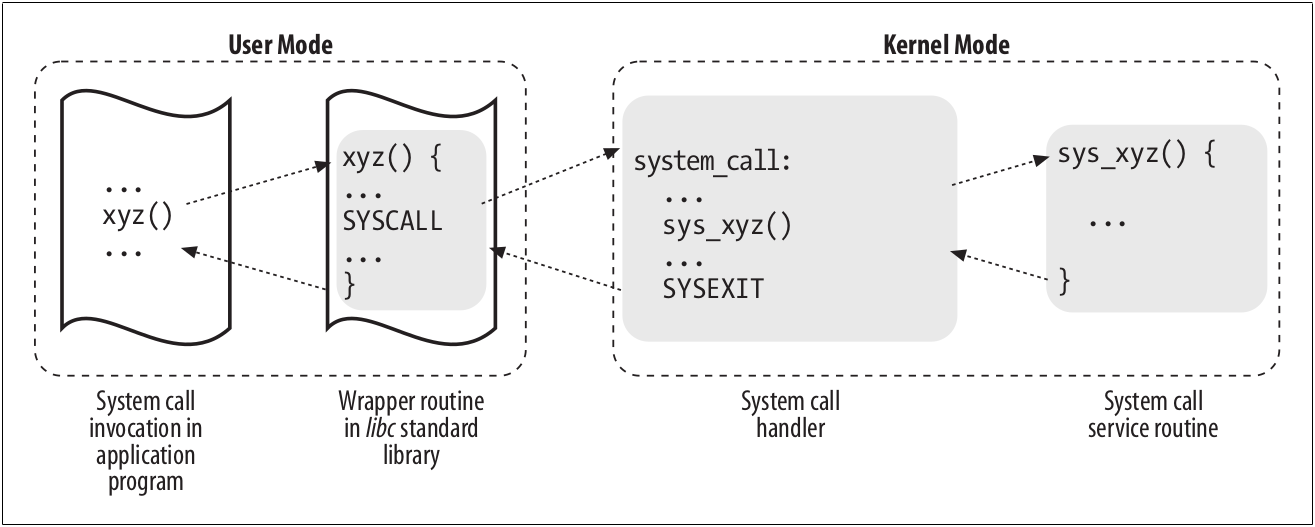
\includegraphics[width=\textwidth]{syscall.png}
  \caption{Общий механизм работы системных вызовов}
  \label{fig:syscall}
\end{figure}

Когда процесс пространства пользователя вызывает системный вызов, процессор
переключается в режим ядра и запускает выполнение функции-обработчика
конкретного системного вызова, что изображено на рисунке~\ref{fig:syscall}.
Более того, даже в пределах ахритектуры системный вызов в Linux может быть
осуществлён несколькими способами. Однако результатом каждого из них является
переход из пользовательской программы к небольшой ассемблерной функции.
Поскольку ядро реализует множество различных системных вызовов, процесс
пользовательского пространства должен передать параметр, представляющий собой
номер системного вызова, для идентификации подставленной перед ядром задачи. Для
этого на архитекктуре х86\_64 используется регистр \texttt{eax}. Бинарный
интерфейс системных вызовов в Linux на каждой из поддерживаемых арихтектур
описан в таблице \ref{table:syscall_abi}.

\begin{table}
  \caption{Бинарный интерфейс системного вызова в Linux}
  \label{table:syscall_abi}
  \begin{tabular}{| >{\raggedright}m{0.18\textwidth}
                  | >{}m{0.28\textwidth}
                  | >{}m{0.11\textwidth}
                  | >{}m{0.18\textwidth}
                  | >{\arraybackslash}m{0.11\textwidth}|}
    \hline
    Архитектура & Инструкция & Регистр номера вызова & Регистр c возвращаемым значением & Регистр ошибки \\ \hline
    alpha & callsys & v0 & a0 & a3 \\ \hline
    arc & trap0 & r8 & r0 & - \\ \hline
    arm/OABI & swi NR & - & a1 & - \\ \hline
    arm/EABI & swi 0x0 & r7 & r0 & - \\ \hline
    arm64 & svc \#0 & x8 & x0 & - \\ \hline
    blackfin & excpt 0x0 & P0 & R0 & - \\ \hline
    i386 & int \$0x80 & eax & eax & - \\ \hline
    ia64 & break 0x100000 & r15 & r8 & r10 \\ \hline
    m68k & trap \#0 & d0 & d0 &  - \\ \hline
    microblaze & brki r14,8 & r12 & r3 & - \\ \hline
    mips & syscall & v0 & v0 & a3 \\ \hline
    nios2 & trap & r2 & r2 & r7 \\ \hline
    parisc & ble 0x100(\%sr2, \%r0) & r20 & r28 & - \\ \hline
    powerpc & sc & r0 & r3 & r0 \\ \hline
    s390 & svc 0 & r1 & r2 & - \\ \hline
    s390x & svc 0 & r1 & r2 & - \\ \hline
    superh & trap \#0x17 & r3 & r0 & - \\ \hline
    sparc/32 & t 0x10 & g1 & o0 & psr/csr \\ \hline
    sparc/64 & t 0x6d & g1 & o0 & psr/csr \\ \hline
    tile & swint1 & R10 & R00 & R01 \\ \hline
    x86\_64 & syscall & rax & rax & - \\ \hline
    x32 & syscall & rax & rax & - \\ \hline
    xtensa & syscall & a2 & a2 & - \\ \hline
  \end{tabular}
\end{table}

Все системные вызовы возвращают целочисленное значение типа \texttt{long}.
Способ предачи возвращаемых значений может отличаться от того, как это делается
в функции обертки. В ядре положительные или нулевые значения обозначают успешное
завершение системного вызова, а отрицательные значения, если это не ядерный
адрес~--- ошибку. В таком случае это значение, которое должно быть возвращено в
программу пользователя в переменной \texttt{errno}. Переменная errno не
установливается и не используется ядром. Вместо этого стандартная библиотека
языка Си обрабатывает возвращенное из ядра значение, установливая параменную
\texttt{errno} для текущего потока.

Рассмотрим механизм работы общего обработчика системного вызова на архитектуре
x86\_64. Он имеет структуру, аналогичную структуре любого другого исключения и
осуществляет следующие операции:
\begin{itemize}
\item cохраняет содержимое большинства регистров на стеке в режиме ядра
  (реализуется на языке ассемблера);
\item меняет отображения страниц для защиты от уязвимостей спекулятивного
  исполнения инструкций;
\item вызывает написанную на Си часть, общую для всех архитектур, откуда в
  последствии вызывается функция-обработчик конкретного вызова;
\item при выходе из обработчика в ассемблерную часть регистры загружаются ранее
  сохранёнными значениями, а процессор переключается из режима ядра в
  пользовательский режим.
\end{itemize}

Переход в режим ядра для системного вызова на архитектуре \texttt{x86\_64} может
осуществляться несколькими способами: исуществлением 80-го программного
прерывания, инструкцией \texttt{sysenter} и инструкцией \texttt{syscall}.
Последний вариант является наиболее актуальным, быстрым и надежным.

При исполнении инструкции \texttt{syscall} процессор переключает уровень
привелегий на нулевое кольцо и осуществляет вызов по виртуальному адресу,
расположенному в регистре IA32\_LSTAR MSR. При этом изменяется значение
регистров \texttt{rcx} и \texttt{r11}, так как для правильного возврата из
пространства ядра адрес возврата помещается на время выполнения вызова в
\texttt{rcx}, а в \texttt{r11} помещается значение регистра флагов
\texttt{rflags}.

Чтобы связать каждый номер системного вызова с его соответствующим обработчиком,
ядро использует таблицу диспетчеризации системных вызовов, которая хранится в
массиве \texttt{sys\_call\_table} с размером, равным \texttt{NR\_syscalls}.
Макрос \texttt{NR\_syscalls}~--- это статический предел максимального количества
элементов в массиве; в целом он не указывает на количество системных вызовов,
однако на \texttt{x86\_64} их значения совпадают, ведь значение макроса
определяется в момент компиляции, и не задается разработчиками напрямую, в
отличие, например, от архитектур PowerPC или IA64. Каждая запись таблицы
диспетчеризации может содержать адрес функции \texttt{sys\_ni\_syscall}, которая
просто возвращает код ошибки \texttt{-ENOSYS}.

Параметры обычных функций в Си обычно передаются путем записи их значений в стек
(либо стек пользовательского режима, либо стек режима ядра). Поскольку системные
вызовы~--- особые функции, переходящий из реэима пользователя в ядро, не может
использоваться ни стек режима пользователя, ни стек режима ядра. Поэтому
передаваемые системному вызову параметры записываются в регистры процессара
перед исполнением. Затем ядро копирует параметры, хранящиеся в регистрах, в
ядерный стек перед вызовом общего обработчика системных вызовов на Си.

Параметры не копируются напрямую из стека режима пользователя в стек ядра по
нескольким причинам. Во-первых, работа с двумя стеками одновременно сложна.
Во-вторых, использование регистров делает структуру обработчика системных
вызовов аналогичной структуре других обработчиков исключений. Однако для
передачи параметров через регистры необходимо выполнять два условия:
\begin{itemize}
\item длина каждого параметра не может превышать длину регистра;
\item количество параметров не должно быть больше шести не считая номер
  системного вызова, переданного в \texttt{eax}, потому что количество регистров
  ограничено.
\end{itemize}

Первое условие всегда выполняется, потому что по стандарту POSIX большие
параметры, которые не могут быть переданы через 32-разрядный регистр, должны
передаваться по указателю. Типичным примером является системный вызов
\texttt{settimeofday()}, который использует структуру с 64-битными значениями.

Однако существуют системные вызовы, для которых требуется больше шести
параметров. В таких случаях один регистр используется как указатель на струтуру
в адресном пространстве процесса, которая содержит значения дополнительных
параметров. При этом, программистам не нужно заботиться об этом обходном пути.
Как и при каждом вызове функции C, параметры автоматически сохраняются в стеке,
а платформозависимая ассемблерная прослойка между обработчиком вызова и входом в
режим ядра сам осуществит подходящий способ передать параметры ядру.

В некоторых случаях, даже если системный вызов не использует напрямую какие-либо
параметры и содержащие их регистры, соответствующий обработчик должен знать
содержимое регистров процессора прямо перед осуществлением системного вызова.
Например, функция \texttt{copy\_thread\_tls()} использующаяся в реализации системного
вызова \texttt{fork()}, должна знать значения регистров, чтобы дублировать их в
дочернем процессе. В этих случаях они достаются с помощью макроса \texttt{current\_pt\_regs}.

Все параметры системного вызова должны быть тщательно проверены до того, как
ядро попытается выполнить требования пользовательской программы. Тип проверки
зависит как от системного вызова, так и от конкретного параметра. Например, в
системном вызове \texttt{write()} параметр \texttt{fd} должен быть файловым
дескриптором, который идентифицирует конкретный файл, поэтому
\texttt{sys\_write()} должен проверить, действительно ли \texttt{fd} является
файловым дескриптором ранее открытого файла и есть ли у процесса процесса права
записи в него. Если какое-либо из этих условий неверно, обработчик должен
вернуть отрицательное значение, в этом случае, код ошибки \texttt{-EBADF}.
Однако один тип проверки является общим для всех системных вызовов. Всякий раз,
когда параметр является адресом, ядро должно проверить, находится ли оно в
адресном пространстве процесса. Существует два возможных способа выполнить эту
проверку:
\begin{itemize}
\item убедиться, что адрес принадлежит адресному пространству процесса, и если
  да, то проверить, что для области памяти, в которую указывает адрес, имеет
  соответствующие права доступа;
\item убедиться, что адрес меньше \texttt{PAGE\_OFFSET}, то есть, он не попадает
  в диапазон адресов, зарезервированных для ядра.
\end{itemize}

Ранние версии ядра Linux выполнили первый тип проверки, однано это занимало
много времени, потому что проверка должна была выполняться для каждого
параметра-адреса, включенного в системный вызов, кроме того, это обычно это
имело мало отдачи, потому что ошибочные программы не очень распространены.
Поэтому, с определенного времени Linux использует второй тип проверки. Это
намного эффективнее, хотя и очевидно, что это очень грубая проверка: проверка
того, что адрес меньше \texttt{PAGE\_OFFSET}, является необходимым, но не
достаточным условием. Таким образом, при втором подходе реальная проверка не
должна осуществляться до последнего возможного момента, то есть до тех пор, пока
виртуальный адрес не будет переведет в физический. Для этого, вместо свободного
доступа к памяти пользовательской программы используются специальные функции,
осуществляющие все необходимые проверки. Основными такими функциями,
используемыми в разработанных системных вызовах, являются:
\begin{itemize}
\item \texttt{copy\_to\_user}~--- копирование произвольного числа байт в
  пространство пользователя;
\item \texttt{copy\_from\_user}~--- копирование произовального числа байт из
  пользовательского буфера в ядерный;
\item \texttt{get\_user}~--- получение значения переменной, на которую указывает
  пользовательский указатель;
\item \texttt{put\_user}~--- помещение переменной из ядра в пространство
  пользователя по переданному указателю.
\end{itemize}

Функции \texttt{get\_user} и \texttt{put\_user} отличаются тем, что копируют
только небольшие значения, способные поместиться в регистр процессора.
Перечисленные функции существуют с целью дополнительных проверок времени
выполнения, является указатель пользовательским, принадлежит ли он текущему
контексту и есть ли соответствующие права доступа на память по переданному
указателю.
